\documentclass[12pt, twoside]{article}
\input{../preamble}

\fancyhead[LO]{La Scuola d'Italia / Dr.\ Huson / IB Math: Quiz \\* 13 March 2026}
\fancyhead[RO]{\fbox{\begin{minipage}{4cm}\footnotesize First \& Last name:\\[0.5cm]\end{minipage}}}
\fancyfoot[C]{\thepage}

\begin{document}
\subsubsection*{4.19 Quiz: Probability (Algebra)}

\begin{enumerate}[itemsep=0.15cm]

%--- Problem 1: Independence with algebra ---
\item Events $A$ and $B$ are independent. It is given that
      $\mathrm{P}(A) = 2\,\mathrm{P}(B)$ and $\mathrm{P}(A \cup B) = 0.72$.

      Let $x = \mathrm{P}(B)$.

\begin{enumerate}[itemsep=0.1cm]
  \item Show that $2x^{2} - 3x + 0.72 = 0$. \hfill [3]
  \item Hence find $\mathrm{P}(B)$. \hfill [2]
  \item Find $\mathrm{P}(A \cap B)$. \hfill [1]
\end{enumerate}

\begin{tikzpicture}
  \draw (-0.6,0) rectangle (11,13);
  \foreach \y in {1,2,...,12} \draw[dotted] (0,\y)--(10.5,\y);
\end{tikzpicture}

\newpage

%--- Problem 2: Conditional probability + Venn ---
\item In a school, 80 students were surveyed about activities $A$ and $B$.

\begin{itemize}[itemsep=0.1cm]
  \item $\mathrm{P}(A) = 0.5$
  \item $\mathrm{P}(B \mid A) = 0.3$
  \item $\mathrm{P}(A' \cap B') = 0.2$
\end{itemize}

\begin{enumerate}[itemsep=0.1cm]
  \item Find $\mathrm{P}(A \cap B)$. \hfill [2]
  \item Find $\mathrm{P}(B)$. \hfill [2]
  \item Complete the Venn diagram below, showing the number
        of students \\in each region. \hfill [2]
  \item Determine whether events $A$ and $B$ are independent.
        Justify your answer. \hfill [2]
\end{enumerate}

\begin{center}
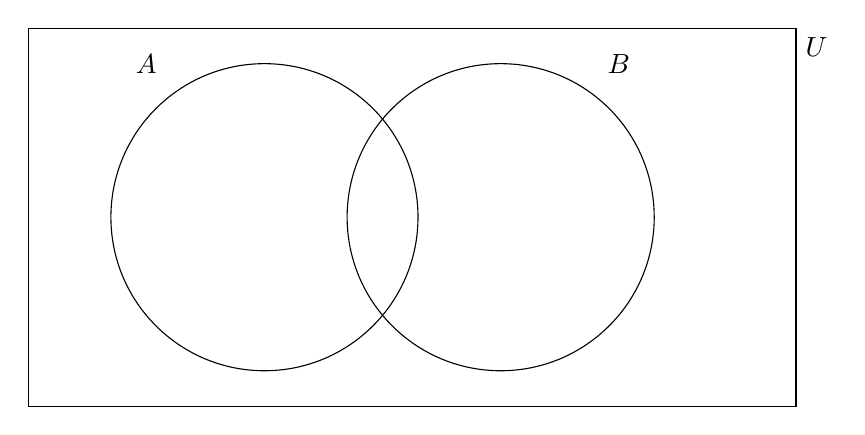
\begin{tikzpicture}[scale=1.5]
  \draw (0,0) rectangle (6.5,3.2);
  \draw (2.0,1.6) circle (1.3);
  \draw (4.0,1.6) circle (1.3);
  \node at (1.0,2.9) {$A$};
  \node at (5.0,2.9) {$B$};
  \node[anchor=north west] at (6.5,3.2) {$U$};
\end{tikzpicture}
\end{center}

\begin{tikzpicture}
  \draw (-0.6,0) rectangle (11,6);
  \foreach \y in {1,2,...,5} \draw[dotted] (0,\y)--(10.5,\y);
\end{tikzpicture}

\end{enumerate}
\end{document}

Solutions
  Problem 1 — Independence + algebra:
  - (a) P(A∪B) = P(A) + P(B) - P(A∩B)
        Since independent: P(A∩B) = P(A)·P(B) = 2x · x = 2x²
        So: 2x + x - 2x² = 0.72 → 3x - 2x² = 0.72 → 2x² - 3x + 0.72 = 0
  - (b) Quadratic formula: x = (3 ± √(9-5.76))/4 = (3 ± √3.24)/4 = (3 ± 1.8)/4
        x = 1.2 (reject, probability > 1) or x = 0.3
        P(B) = 0.3
  - (c) P(A∩B) = P(A)·P(B) = 0.6 × 0.3 = 0.18

  Problem 2 — Conditional probability + Venn:
  - (a) P(A∩B) = P(B|A)·P(A) = 0.3 × 0.5 = 0.15
  - (b) P(A∪B) = 1 - P(A'∩B') = 1 - 0.2 = 0.8
        P(B) = P(A∪B) - P(A) + P(A∩B) = 0.8 - 0.5 + 0.15 = 0.45
  - (c) Venn: A only = 28, A∩B = 12, B only = 24, neither = 16. Total = 80 ✓
  - (d) P(A)·P(B) = 0.5 × 0.45 = 0.225 ≠ 0.15 = P(A∩B) → not independent
